%%%%%%%%%%%%%%%%%%%%%%%%%%%%%%%%%%%%%%%%%
% Beamer Presentation
% LaTeX Template
% Version 1.0 (10/11/12)
%
% This template has been downloaded from:
% http://www.LaTeXTemplates.com
%
% License:
% CC BY-NC-SA 3.0 (http://creativecommons.org/licenses/by-nc-sa/3.0/)
%
%%%%%%%%%%%%%%%%%%%%%%%%%%%%%%%%%%%%%%%%%

%----------------------------------------------------------------------------------------
%	PACKAGES AND THEMES
%----------------------------------------------------------------------------------------

\documentclass[presentation]{beamer}

% The Beamer class comes with a number of default slide themes
% which change the colors and layouts of slides. Below this is a list
% of all the themes, uncomment each in turn to see what they look like.

%\usetheme{default}
%\usetheme{AnnArbor}
%\usetheme{Antibes}
%\usetheme{Bergen}
% \usetheme{Berkeley}
% \usetheme{Berlin}
%\usetheme{Boadilla}
%\usetheme{CambridgeUS}
%\usetheme{Copenhagen}
%\usetheme{Darmstadt}
% \usetheme{Dresden}
%\usetheme{Frankfurt}
%\usetheme{Goettingen}
%\usetheme{Hannover}
%\usetheme{Ilmenau}
%\usetheme{JuanLesPins}
%\usetheme{Luebeck}
\usetheme{Madrid}
%\usetheme{Malmoe}
%\usetheme{Marburg}
%\usetheme{Montpellier}
%\usetheme{PaloAlto}
%\usetheme{Pittsburgh}
%\usetheme{Rochester}
%\usetheme{Singapore}
%\usetheme{Szeged}
%\usetheme{Warsaw}

% As well as themes, the Beamer class has a number of color themes
% for any slide theme. Uncomment each of these in turn to see how it
% changes the colors of your current slide theme.

%\usecolortheme{albatross}
%\usecolortheme{beaver}
%\usecolortheme{beetle}
%\usecolortheme{crane}
%\usecolortheme{dolphin}
%\usecolortheme{dove}
%\usecolortheme{fly}
%\usecolortheme{lily}
%\usecolortheme{orchid}
%\usecolortheme{rose}
%\usecolortheme{seagull}
%\usecolortheme{seahorse}
%\usecolortheme{whale}
%\usecolortheme{wolverine}

%\setbeamertemplate{footline} % To remove the footer line in all slides uncomment this line
%\setbeamertemplate{footline}[page number] % To replace the footer line in all slides with a simple slide count uncomment this line

\setbeamertemplate{navigation symbols}{} % To remove the navigation symbols from the bottom of all slides uncomment this line

\usepackage{graphicx} % Allows including images
\usepackage{booktabs} % Allows the use of \toprule, \midrule and \bottomrule in tables
\usepackage{textpos}

\title[Improved Modern Hopfield Network]{Improved Robustness and Hyperparameter Selection in the Modern Hopfield Network}
\author[School of Computing]{Hayden McAlister} 
\institute[]{
% \includegraphics[scale=0.25]{}
School of Computing, University of Otago
}
\date{Supervisors: Anthony Robins, Lech Syzmanski} 

%----------------------------------------------------------------------------------------
%	TITLE PAGE 1
%----------------------------------------------------------------------------------------
\begin{document}

\begin{frame}
\titlepage % Print the title page as the first slide
\end{frame}


%----------------------------------------------------------------------------------------
%	TITLE PAGE
%----------------------------------------------------------------------------------------

\begin{frame}
\frametitle{Overview} 
\tableofcontents 
\end{frame}

% --------------------------------------------------------------------------------

\section{Introduction} 

\begin{frame}
	
\frametitle{Autoassociative Memories}

\begin{itemize}
    \item Learn to associate a state with itself.
    \item Relax probe towards a learned state.
\end{itemize}

\only<1> {
    \begin{center}
        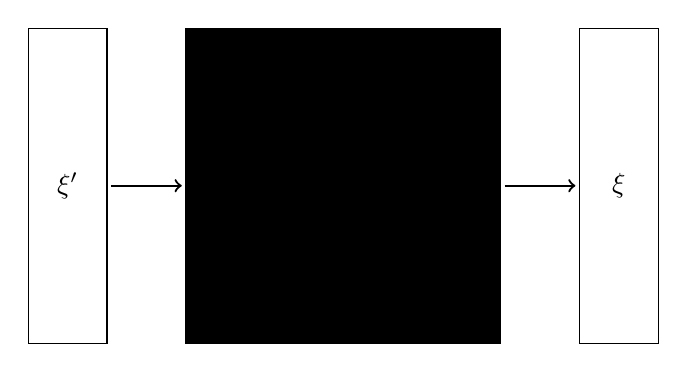
\begin{tikzpicture}
            \draw (0,0) rectangle (1,4);
            \node at (0.5,2) {$\xi^\prime$};
            \draw[thick, ->] (1.05,2) --(1.95,2);
        
            \filldraw[fill=\fillColor, draw=black] (2,0) rectangle (6,4);
            \node[align=center] at (4,2) {Autoassociative\\Memory};
            
            \draw (7,0) rectangle (8,4);
            \node at (7.5,2) {$\xi$};
            \draw[thick, ->] (6.05,2) --(6.95,2);
        \end{tikzpicture}
    \end{center}
}



% \only<1>{
% \begin{center}
% \begin{tikzpicture}
%     \draw (0,0) rectangle (1,4);
%     \node at (0.5,2) {$\xi$};
%     \draw[thick, ->] (1.05,2) --(1.95,2);

%     \filldraw[fill=\fillColor, draw=black] (2,0) rectangle (6,4);
%     \node[align=center] at (4,2) {Autoassociative\\Memory};
    
%     \draw (7,0) rectangle (8,4);
%     \node at (7.5,2) {$\xi$};
%     \draw[thick, ->] (6.05,2) --(6.95,2);
% \end{tikzpicture}
% \end{center}
% }

% \only<2>{
% \begin{center}
%     \begin{tikzpicture}
%         \draw (0,0) rectangle (1,4);
%         \node at (0.5,2) {$\xi$};
%         \draw[thick, ->] (1.05,2) --(1.95,2);
    
%         \filldraw[fill=\fillColor, draw=black] (2,0) -- (4,1.5) -- (4,2.5) --(2,4) -- (2,0);
%         \filldraw[fill=\fillColor, draw=black] (4,1.5) -- (4,2.5) -- (6,4) -- (6,0) -- (4, 1.5);
        
%         \draw (7,0) rectangle (8,4);
%         \node at (7.5,2) {$\xi$};
%         \draw[thick, ->] (6.05,2) --(6.95,2);
%     \end{tikzpicture}
% \end{center}
% }

% \only<3>{
% \begin{center}
%     \begin{tikzpicture}
%         \draw (0,0) rectangle (1,4);
%         \node at (0.5,2) {$\xi$};

%         \draw[thick, ->] (1.05,2) --(6.95,2);
        
%         \draw (7,0) rectangle (8,4);
%         \node at (7.5,2) {$\xi$};
%     \end{tikzpicture}
% \end{center}
% }

% \only<4>{
% \begin{center}
% \begin{tikzpicture}
%     \draw (0,0) rectangle (1,4);
%     \node at (0.5,2) {$\xi^\prime$};
%     \draw[thick, ->] (1.05,2) --(1.95,2);

%     \filldraw[fill=\fillColor, draw=black] (2,0) rectangle (6,4);
%     \node[align=center] at (4,2) {Autoassociative\\Memory};
    
%     \draw (7,0) rectangle (8,4);
%     \node at (7.5,2) {$\xi$};
%     \draw[thick, ->] (6.05,2) --(6.95,2);
% \end{tikzpicture}
% \end{center}
% }
    
\end{frame}

% --------------------------------------------------------------------------------

\subsection{Classical Hopfield Network} 

\begin{frame}
\frametitle{Classical Hopfield Network}

\only<1> {
    \begin{center}
    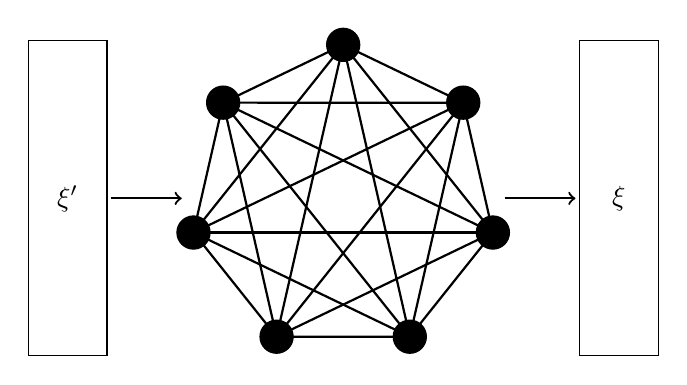
\begin{tikzpicture}
        \draw (0,0) rectangle (1,4);
        \node at (0.5,2) {$\xi^\prime$};
        \draw[thick, ->] (1.05,2) --(1.95,2);
        
        \pgfmathtruncatemacro{\numNodes}{7}
        \pgfmathsetmacro{\networkRadius}{1.95}
        \foreach \t in {1,...,\numNodes}{
            \foreach \u in {\t,...,\numNodes} {
                \draw[thick, ->] ({\networkRadius * sin(360 / \numNodes * \t)+4},{\networkRadius * cos(360 / \numNodes * \t)+2}) --({\networkRadius * sin(360 / \numNodes * \u)+4},{\networkRadius * cos(360 / \numNodes * \u)+2});
            }
            \filldraw [fill=\fillColor, draw=black] ({\networkRadius * sin(360 / \numNodes * \t)+4},{\networkRadius * cos(360 / \numNodes * \t)+2}) circle (6pt);
        }
        
        \draw (7,0) rectangle (8,4);
        \node at (7.5,2) {$\xi$};
        \draw[thick, ->] (6.05,2) --(6.95,2);
    \end{tikzpicture}
    \end{center}
}

\only<2>{    
    \begin{columns}[c]
        \column{.6\textwidth}
        \begin{itemize}
            \item Association by Hebbian learning.
            \begin{itemize}
                \item Biological inspiration.
                \item Easy to analyze.
            \end{itemize}
            \item Relax by matrix multiplication.
            \begin{itemize}
                \item Mean field approximation.
                \item Nonlinearity keeps states in bipolar domain.
                \item Energy guaranteed to achieve a minima (under sensible conditions).
            \end{itemize}
        \end{itemize}

        \column{.4\textwidth}
        % TODO Classical Hopfield Image
        \begin{align}
            W &= \sum_{k} \xi_k \otimes \xi_k \\
            \xi_{t+1} &= \text{ Sign}\left( W \cdot \xi_{t} \right) \\
            E \left( \xi \right) &= -\frac{1}{2} \xi^T W \xi
        \end{align}
    \end{columns}
}
\end{frame}

% --------------------------------------------------------------------------------

\subsection{Modern Hopfield Network} 

\begin{frame}
	
    \frametitle{Modern Hopfield Network}
    \begin{columns}[c]
        \column{.6\textwidth}
        \begin{itemize}
            \item Classical energy wells are too shallow.          
        \end{itemize}
        
        

        \column{.4\textwidth}
        \only<1>{
            \begin{figure}[h]
                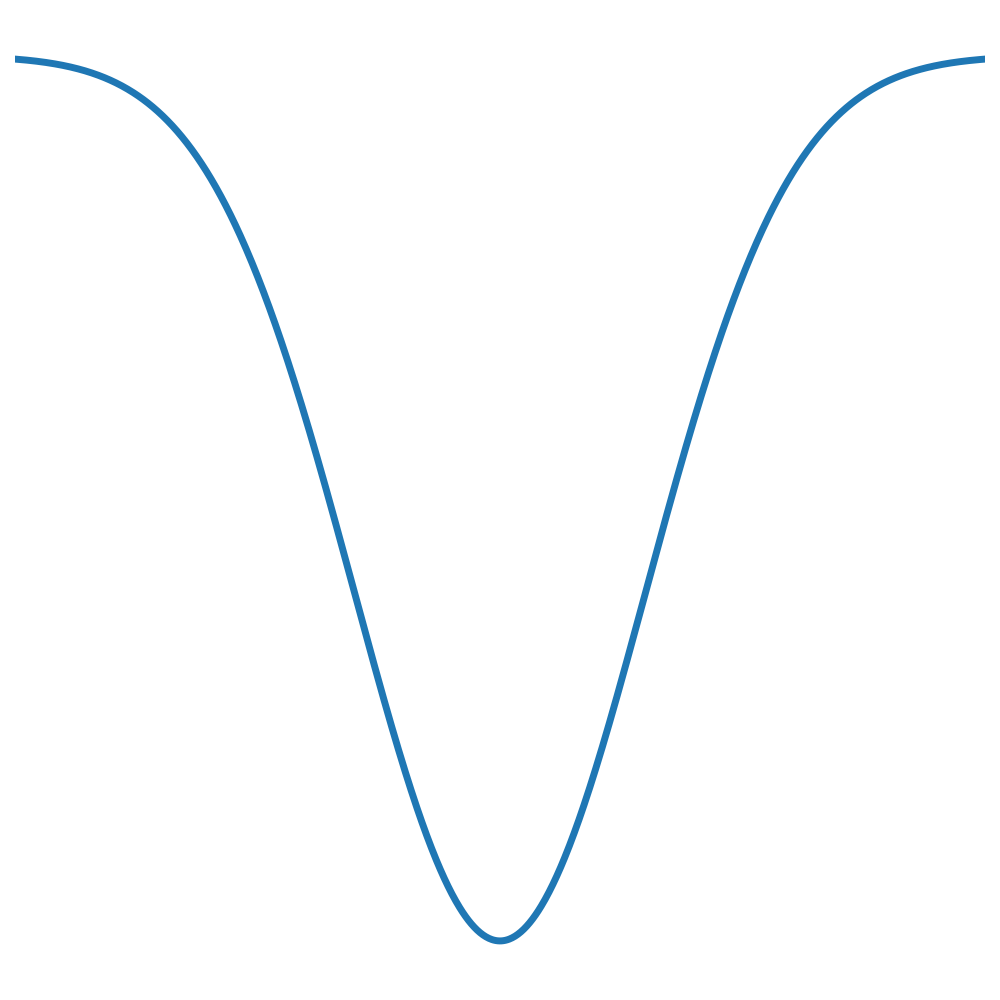
\includegraphics[width=\textwidth]{images/introduction_energywell01.png}
            \end{figure}
        }
        \only<2>{
            \begin{figure}[h]
                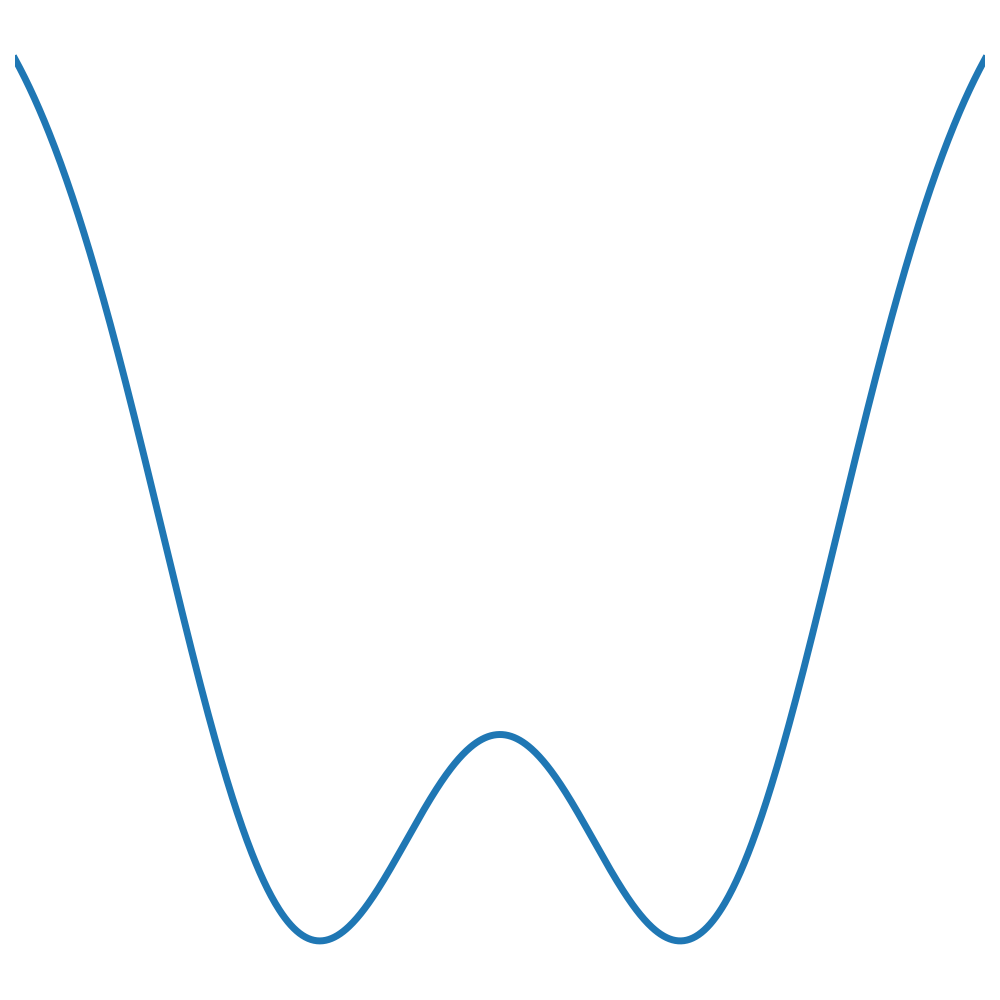
\includegraphics[width=\textwidth]{images/introduction_energywell02.png}
            \end{figure}
        }
        
    \end{columns}
\end{frame}

% --------------------------------------------------------------------------------

\begin{frame}
    \frametitle{Modern Hopfield Network}
    \begin{columns}[c]
        \column{.6\textwidth}
        \begin{itemize}
            \item Key trick: Replace quadratic energy with general polynomial.
            \begin{itemize}
                \item Heck, anything with a vaguely polynomial shape.
            \end{itemize}
        \end{itemize}

        \begin{align*}
            f_n\left( x \right) &= x^n \\
            f_n\left( x \right) &= \begin{cases}
                x^n \; \text{if } x\geq0 \\
                0 \; \text{if } x<0
            \end{cases} \\
            f_n\left( x \right) &= \begin{cases}
                x^n \; \text{if } x\geq0 \\
                -\epsilon x \; \text{if } x<0
            \end{cases}
        \end{align*}

        \column{.4\textwidth}
        \begin{figure}[h]
            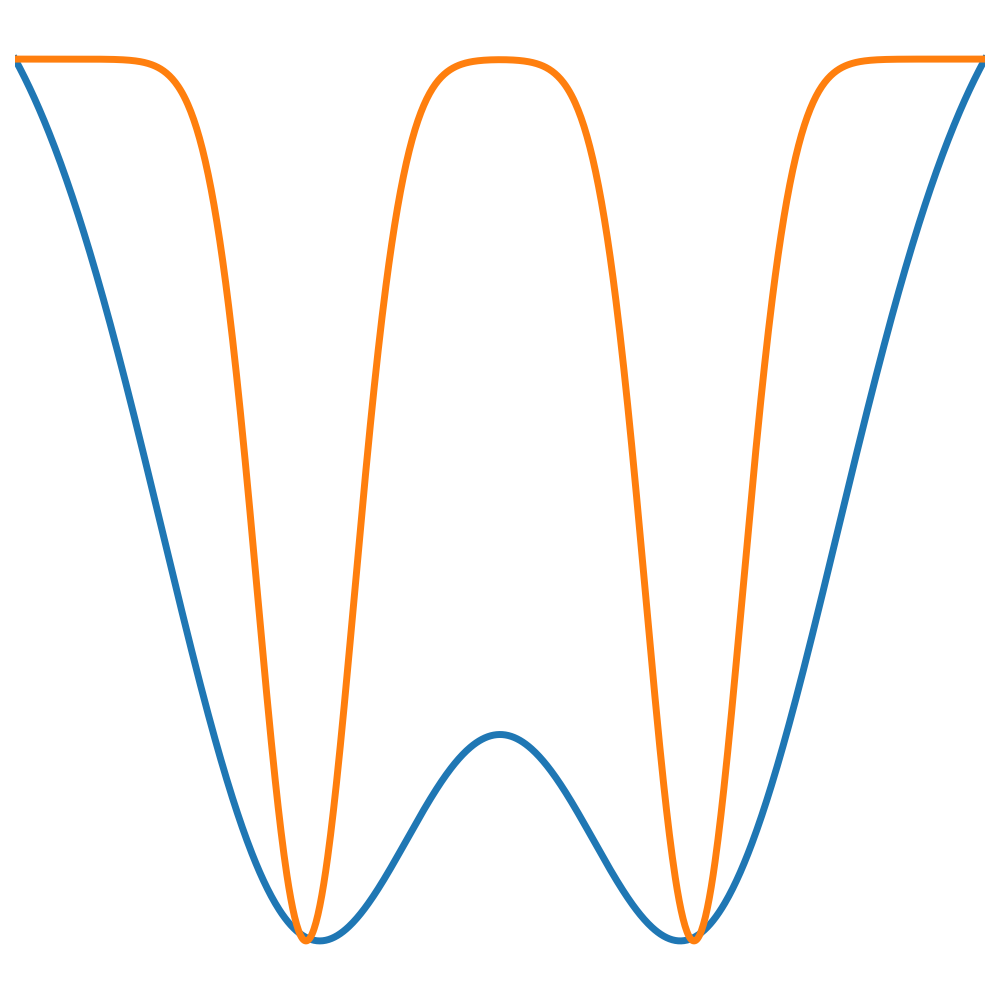
\includegraphics[width=\textwidth]{images/introduction_energywell03.png}
        \end{figure}
    \end{columns}
\end{frame}

% --------------------------------------------------------------------------------

\begin{frame}[t]
	
    \frametitle{Modern Hopfield Network}
    
    \begin{block}{\(n\) -- The Interaction Vertex}
        \begin{itemize}
            \item Controls the range of influence that memories have.
            \item However, also radically alters the network architecture.
        \end{itemize}
    \end{block}

        \only<1>{
            Memory matrix replaced by list of memory states -- vectors of same dimension as data.
            
            \begin{center}
                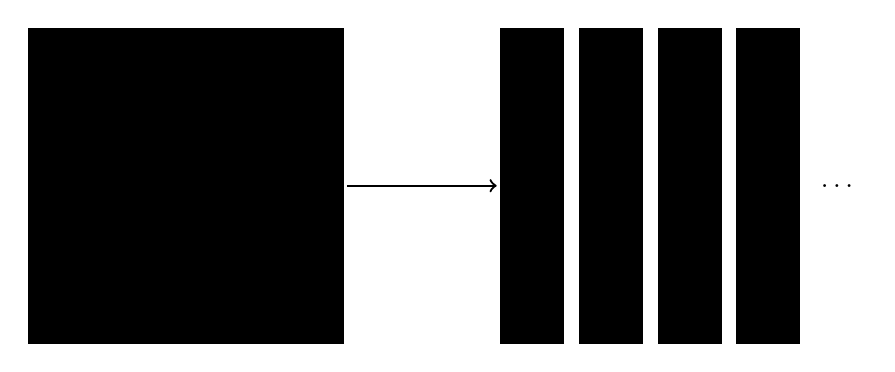
\begin{tikzpicture}
                    \filldraw[fill=\fillColor, draw=black] (0,0) rectangle (4,4);
                    \node at (2,2) {$\xi \otimes \xi$};
                    
                    \draw[thick, ->] (4.05, 2) -- (5.95, 2);
                    \filldraw[fill=\fillColor, draw=black] (6,0) rectangle (6.8,4);
                    \node at (6.4, 2) {$\zeta_0$};
                    \filldraw[fill=\fillColor, draw=black] (7,0) rectangle (7.8,4);
                    \node at (7.4, 2) {$\zeta_1$};
                    \filldraw[fill=\fillColor, draw=black] (8,0) rectangle (8.8,4);
                    \node at (8.4, 2) {$\zeta_2$};
                    \filldraw[fill=\fillColor, draw=black] (9,0) rectangle (9.8,4);
                    \node at (9.4, 2) {$\zeta_3$};
                    \node at (10.3, 2) {\dots};
                \end{tikzpicture}
            \end{center}
        }
        
        \only<2>{
            Relaxation no longer uses mean field -- now a contrastive difference.
            \begin{itemize}
                \item Negative energy no longer means ``stable'' -- the energy \textit{difference} between a neuron clamped on and off indicates stability.
            \end{itemize}

            \begin{center}
                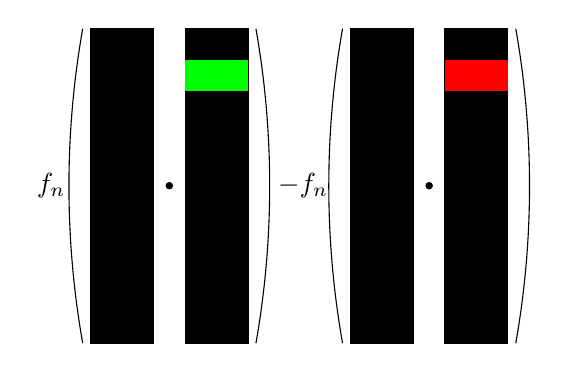
\begin{tikzpicture}
                    \node at (-0.5, 2) {$f_n$};
                    \draw (-0.1, 0) arc (190:170:11.5);
                    \filldraw[fill=\fillColor, draw=black] (0,0) rectangle (0.8,4);
                    \node at (0.4, 2) {$\zeta$};
                    
                    \filldraw (1, 2) circle (0.04);
                    
                    \filldraw[fill=\fillColor, draw=black] (1.2,0) rectangle (2,4);
                    \fill[fill=green] (1.2,3.2) rectangle (2,3.6);
                    \node at (1.6, 2) {$\xi_{+1}$};
                    \draw (2.1, 0) arc (-10:10:11.5);
                    
                    \node at (2.7, 2) {$- f_n$};
                    \draw (3.2, 0) arc (190:170:11.5);

                    \filldraw[fill=\fillColor, draw=black] (3.3,0) rectangle (4.1,4);
                    \node at (3.7, 2) {$\zeta$};

                    \filldraw (4.3, 2) circle (0.04);
                    
                    \filldraw[fill=\fillColor, draw=black] (4.5,0) rectangle (5.3,4);
                    \fill[fill=red] (4.5,3.2) rectangle (5.3,3.6);
                    \node at (4.9, 2) {$\xi_{-1}$};
                    \draw (5.4, 0) arc (-10:10:11.5);
                \end{tikzpicture}
            \end{center}
            
        }

        \only<3>{
            Learning no longer supports Hebbian -- now requires gradient descent.

            \begin{gather*}
             W = \sum_{k} \xi_k \otimes \xi_k \\
             \text{Loss}\left( \xi \right) = \tanh \left[ \beta \sum_{\mu} \left( f_n \left(\zeta_{\mu, i} + \sum_{j \neq i} \zeta_{\mu, j} \xi_{j} \right) - f_n \left( -\zeta_{\mu, i} + \sum_{j \neq i} \zeta_{\mu, j} \xi_{j} \right) \right) \right]
            \end{gather*}
        }       
    
\end{frame}
\section{Objectives of the Project}
\begin{frame}
	
\frametitle{Objectives}

You may list the objectives here\\~\\


\end{frame}

%------------------------------------------------
\section{Methodology}

\begin{frame}
\frametitle{Methodology}
\begin{itemize}
\item Lorem ipsum dolor sit amet, consectetur adipiscing elit
\item Aliquam blandit faucibus nisi, sit amet dapibus enim tempus eu
\item Nulla commodo, erat quis gravida posuere, elit lacus lobortis est, quis porttitor odio mauris at libero
\item Nam cursus est eget velit posuere pellentesque
\item Vestibulum faucibus velit a augue condimentum quis convallis nulla gravida
\end{itemize}
\end{frame}

%------------------------------------------------
\section{Block level design}
\begin{frame}
\frametitle{Block level design}
\begin{block}{Block 1}
Lorem ipsum dolor sit amet, consectetur adipiscing elit. Integer lectus nisl, ultricies in feugiat rutrum, porttitor sit amet augue. Aliquam ut tortor mauris. Sed volutpat ante purus, quis accumsan dolor.
\end{block}

\begin{block}{Block 2}
Pellentesque sed tellus purus. Class aptent taciti sociosqu ad litora torquent per conubia nostra, per inceptos himenaeos. Vestibulum quis magna at risus dictum tempor eu vitae velit.
\end{block}

\begin{block}{Block 3}
Suspendisse tincidunt sagittis gravida. Curabitur condimentum, enim sed venenatis rutrum, ipsum neque consectetur orci, sed blandit justo nisi ac lacus.
\end{block}
\end{frame}

%------------------------------------------------

\section{Components and or tools used}
\begin{frame}
\frametitle{Components and or tools used}
\begin{columns}[c] % The "c" option specifies centered vertical alignment while the "t" option is used for top vertical alignment

\column{.45\textwidth} % Left column and width
\textbf{Heading}
\begin{enumerate}
\item Statement
\item Explanation
\item Example
\end{enumerate}

\column{.5\textwidth} % Right column and width
Lorem ipsum dolor sit amet, consectetur adipiscing elit. Integer lectus nisl, ultricies in feugiat rutrum, porttitor sit amet augue. Aliquam ut tortor mauris. Sed volutpat ante purus, quis accumsan dolor.

\end{columns}
\end{frame}


%------------------------------------------------
\section{Implementation}
%------------------------------------------------

\begin{frame}
\frametitle{Implementation Data }
\begin{table}
\begin{tabular}{l l l}
\toprule
\textbf{Treatments} & \textbf{Response 1} & \textbf{Response 2}\\
\midrule
Treatment 1 & 0.0003262 & 0.562 \\
Treatment 2 & 0.0015681 & 0.910 \\
Treatment 3 & 0.0009271 & 0.296 \\
\bottomrule
\end{tabular}
\caption{Table caption}
\end{table}
\end{frame}

%------------------------------------------------

\section{Final Results and Prototype}

\begin{frame}
\frametitle{Final Results and Prototype}
\begin{theorem}[Mass--energy equivalence]
$E = mc^2$
\end{theorem}
\end{frame}

%------------------------------------------------


\begin{frame}[fragile] % Need to use the fragile option when verbatim is used in the slide
\frametitle{Verbatim}
\begin{example}[Theorem Slide Code]
\begin{verbatim}
\begin{frame}
\frametitle{Theorem}
\begin{theorem}[Mass--energy equivalence]
$E = mc^2$
\end{theorem}
\end{frame}\end{verbatim}
\end{example}
\end{frame}

%------------------------------------------------

\section{Work plan and task allocation}
\begin{frame}
\frametitle{Work plan and task allocation}
Uncomment the code on this slide to include your own image from the same directory as the template .TeX file.
%\begin{figure}
%\includegraphics[width=0.8\linewidth]{test}
%\end{figure}
\end{frame}

%------------------------------------------------

\section{Conclusion}
\begin{frame}[fragile] % Need to use the fragile option when verbatim is used in the slide
\frametitle{Conclusion}
An example of the \verb|\cite| command to cite within the presentation:\\~

This statement requires citation.
\end{frame}

%------------------------------------------------
\section{References}

\begin{frame}
\frametitle{References}
% \footnotesize{
% \begin{thebibliography}{99} % Beamer does not support BibTeX so references must be inserted manually as below
% \end{thebibliography}
% }
\end{frame}

%------------------------------------------------

%----------------------------------------------------------------------------------------


\end{document} 